


We show some numerical experiments that show how the Newton method converges to the fixed point. 

\subsection{Maximal accuracy}


\subsubsection{Estimating stopping criterion for the non-linear solver}
The accuracy on the Newton-Krylov solution is inevitably limited by the noise on the stochastic coarse-time-stepper, which appears in the evaluation of the residual and in the evaluation of the Jacobian-vector-product. The variance on the coarse-time-stepper is of order $\mathcal{O}(\frac{1}{N})$, as shown in fig. \ref{fig:Variance_on_cts(N-1)}. If we use weighted restriction, the variance on the Jacobian-vector-product converges in the same way.  Therefore, the accuracy on the Newton-Krylov solution will depend on the number of particles $N$ used to calculate the coarse time-stepper.  This is confirmed in fig. \ref{fig:Newton_sde_res(k)}, which shows the convergence of the Newton-residuals. When the Newton-Krylov solution is converged, it stays oscillating around the true solution with a standard deviation depending on the number of particles. Because the solution only depends on the previous density and on the random choices in the coarse time stepper, we can interpret this as a Markov chain. The residual averaged out over the converged Newton iterations is a good indication of the best tolerance we can achieve. It converges as $\mathcal{O}(\frac{1}{\sqrt{N}})$. Given the number of particles $N$,  we will use this tolerance as the stopping criterion for the Newton-method.

\subsubsection{Estimating stopping criterion for the linear solver}
Because the solution of the Newton-Krylov solution will contain noise anyway, it is pointless to iterate the linear solver until reaching machine precision.
In fact, for low particle numbers (and a high variance on the left and right side of the linear equation we need to solve), we observe more failed Newton-iterations if the GMRES-tolerance is chosen too small.  

A question of interest is then `what is a good value for the GMRES-tolerance?'. The answer depends on the desired accuracy of the calculated fixed points. For instance in fig. \ref{fig:Newton_sde_res(k)_tol1e-4}, we observe that we  can already stop the Krylov iterations if the density is calculated to an accuracy of %$\varepsilon_{\texttt{GMRES}}=
$10^{-4}$ when $N \leq 10^7$, but that we need a smaller GMRES-tolerance if a higher accuracy is desired (by using more particles). Therefore, in the simulations we  will use $\varepsilon_{\texttt{GMRES}}= 10/N$.


\begin{figure}[H!]
\centering
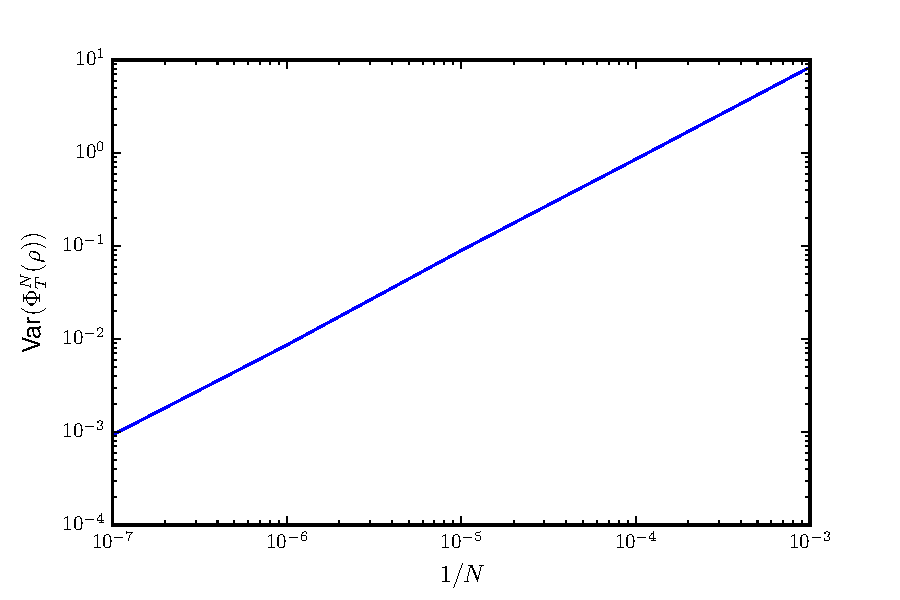
\includegraphics[width=0.49\linewidth]{../Problems/WeightedParticles/checkSystem/plots/Variance_on_cts(N-1)}
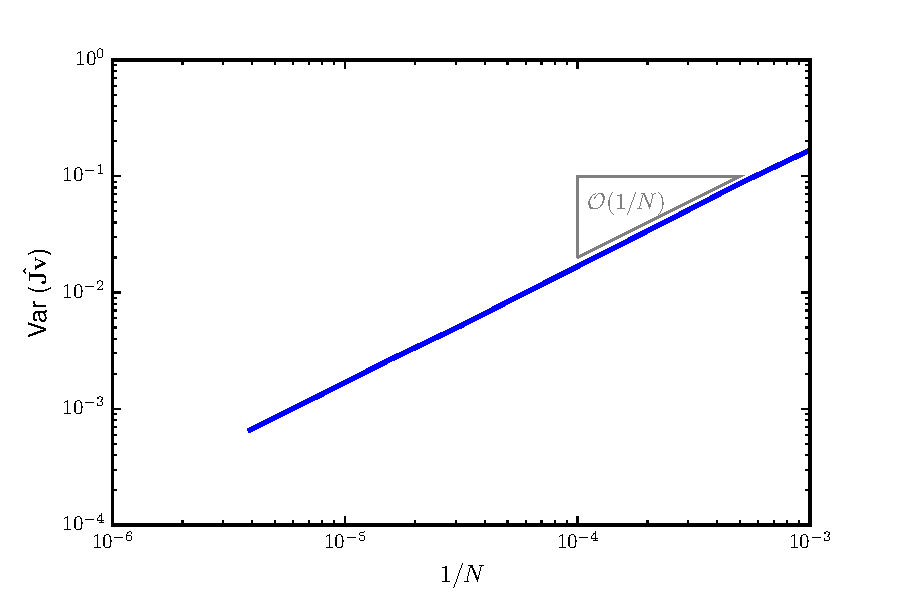
\includegraphics[width=0.49\linewidth]{../Problems/WeightedParticles/checkSystem/plots/Variance_on_Jv}
\caption{The variance of the coarse time-stepper and the variance on the Jacobian vector-product converge to zero with $\mathcal{O}(\frac{1}{N})$ }
\label{fig:Variance_on_cts(N-1)}
\end{figure}



\begin{figure}[H!]
\centering
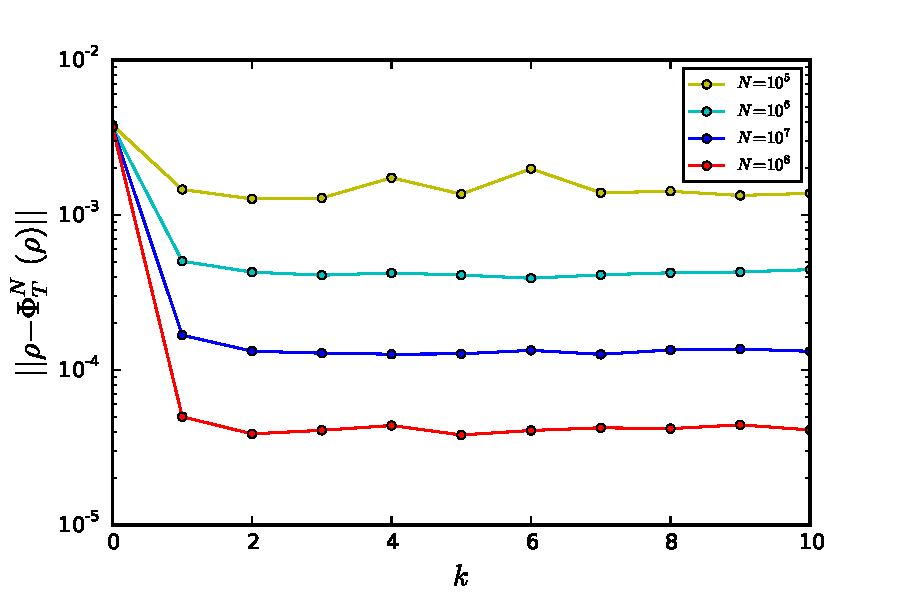
\includegraphics[width=0.5\linewidth]{../Problems/WeightedParticles/checkSystem/Newton/plots/Newton_sde_res(k)_Dt_e-2_tol1e-7.pdf}
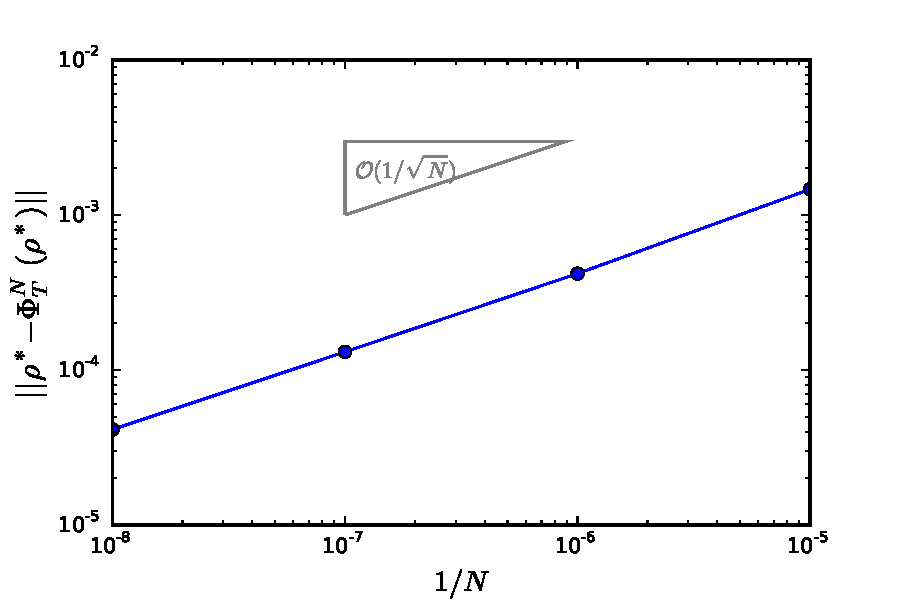
\includegraphics[width=0.49\linewidth]{../Problems/WeightedParticles/checkSystem/Newton/plots/Tolerance_on_NK-solution_converges_N-1_tol_1e-7.pdf}

\caption{ The non-linear solver converges after 1 Newton iteration, up to a tolerance which depends on the number of particles $N$ (\textit{left}). This best achieved tolerance converges to zero with  $\mathcal{O}(\frac{1}{\sqrt{N}})$ (\textit{right}). Parameter values:  $\Delta t = 10^{-3}, \Delta T = 10^{-1} , \epsilon_{\texttt{GMRES}}=10^{-7}$
}.
\label{fig:Newton_sde_res(k)}
\end{figure}

\begin{figure}[H!]
\centering
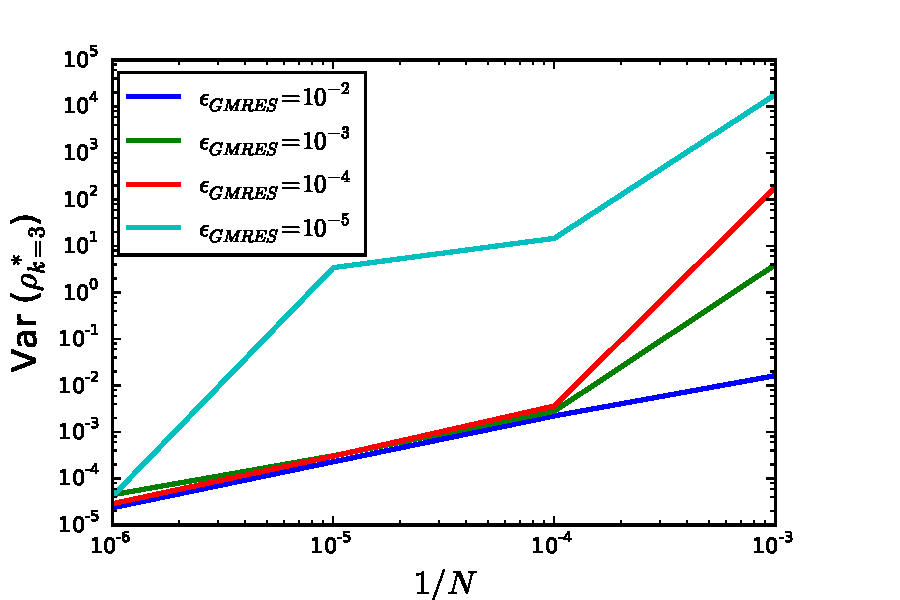
\includegraphics[width=0.32\linewidth]{../Problems/WeightedParticles/checkSystem/plots/Variance_3th_newton_it_Dt1e-1}
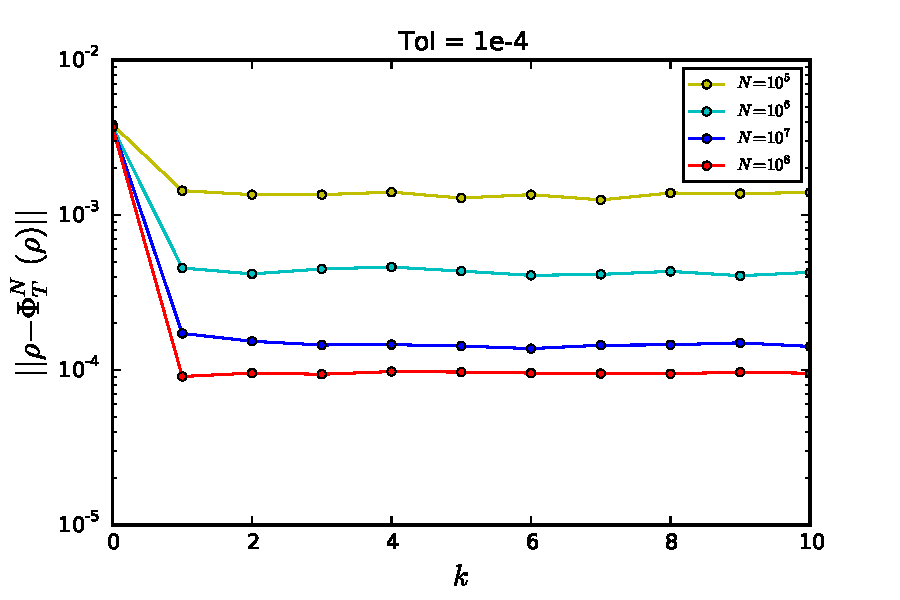
\includegraphics[width=0.32\linewidth]{../Problems/WeightedParticles/checkSystem/Newton/plots/Newton_sde_res(k)_Dt_e-2_tol1e-4}
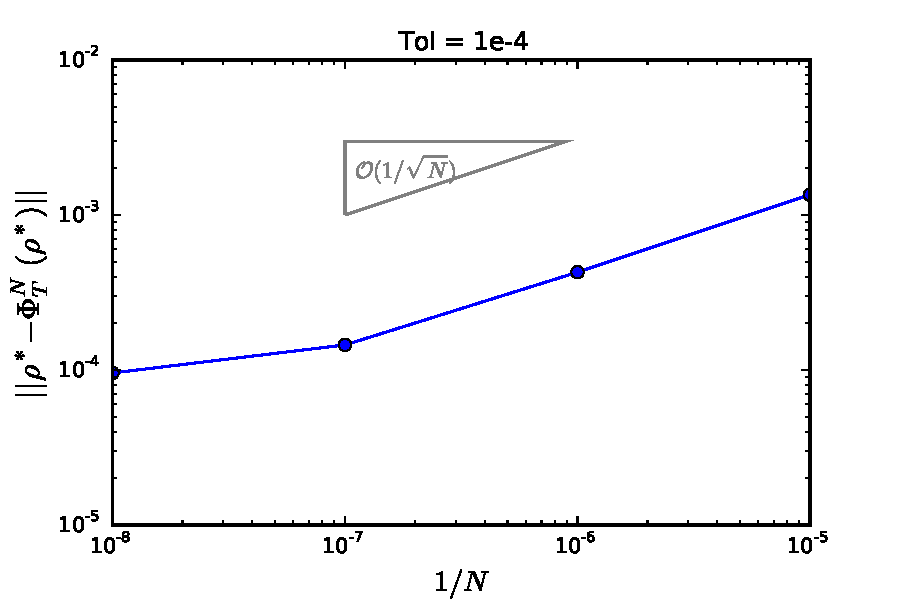
\includegraphics[width=0.32\linewidth]{../Problems/WeightedParticles/checkSystem/Newton/plots/Tolerance_on_NK-solution_converges_N-1_tol_1e-4}

\caption{If the GMRES-tolerance is chosen too small, failed Newton-iterations blew up the variance (in simulations with few particles), as shown in the left plot. However if the GMRES-tolerance is too big, it limits the accuracy of the Newton-Krylov-solver in simulations with many particles. For instance, the best achieved tolerance for $N=10^8$ is limited because of the size of the GMRES-tolerance ($\epsilon_{\texttt{GMRES}}=10^{-4}$), as shown in the two plots on the right.}
\label{fig:Newton_sde_res(k)_tol1e-4}
\end{figure}






%How to cheaply estimate the stopping criterion?

%Is the resulting fixed point biased?
%Can we reduce variance by averaging over a number of 'converged' Newton iterations?
%Additional questions of interest:
%
%Can we stop the Krylov iterations before reaching machine precision (knowing that the end result will contain noise anyway)? 
%
%Does an inaccuracy in the solution of the linear systems increase the required number of Newton iterations?
%
%Do we keep the particles fixed throughout the Newton iterations as well? (We can then probably converge the Newton procedure to machine precision.) What is then the probability distribution of the obtained fixed points? Bias? Variance?

%\subsection{Results for the pde}
%Ook hier zien we dat de keuze van de newtontolerantie belangrijk is (te groot = kans op dezelfde toestanden , te klein= failed iterations).
%Dit kan echter opgevangen worden door de oplossing van dx nauwkeuriger te maken door de tolerantie van de GMRES te verfijnen (het probleem was dat er dx=0 oplossingen werden teruggegeven) 

%\begin{figure}
%%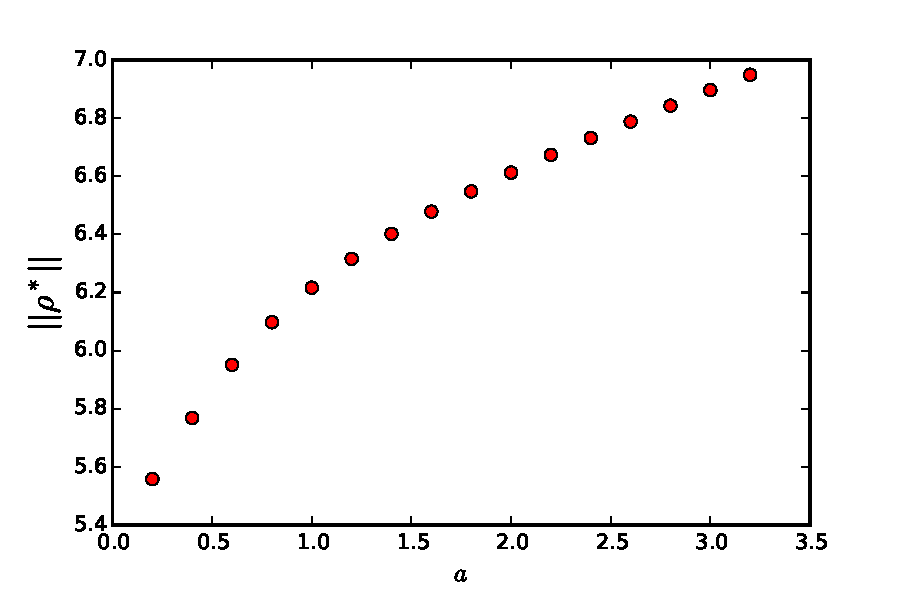
\includegraphics{../Problems/WeightedParticles/checkSystem/plots/bifurcation_pde(D)}
%\caption{  Bifurcation diagram of the steady states calculated with the Newton-Krylov-Solver for the PDE. $\Delta t = 10^{-4}, \Delta T = 10^{-2}, \Delta x = 10^{-2}, \Delta D = 0.01, \epsilon_{GMRES}=10^{-5},  \delta_{Newton} = 10^{-7}, \epsilon=10^{-5}$
%}
%\end{figure}

%\subsection{Results for the sde}


\subsection{Continuation}
 We start from a known solution to the steady-state problem, increment the continuation parameter and solve a new problem using the previous solution as an initial guess. We chose $\Delta \sigma = 0.05$ as continuation step size. Performing a bifurcation with smaller steps is pointless, because the difference in densities will become too small in comparison with the noise on the residual.

\begin{figure}[h]
\centering
%\begin{subfigure}{0.5\textwidth}
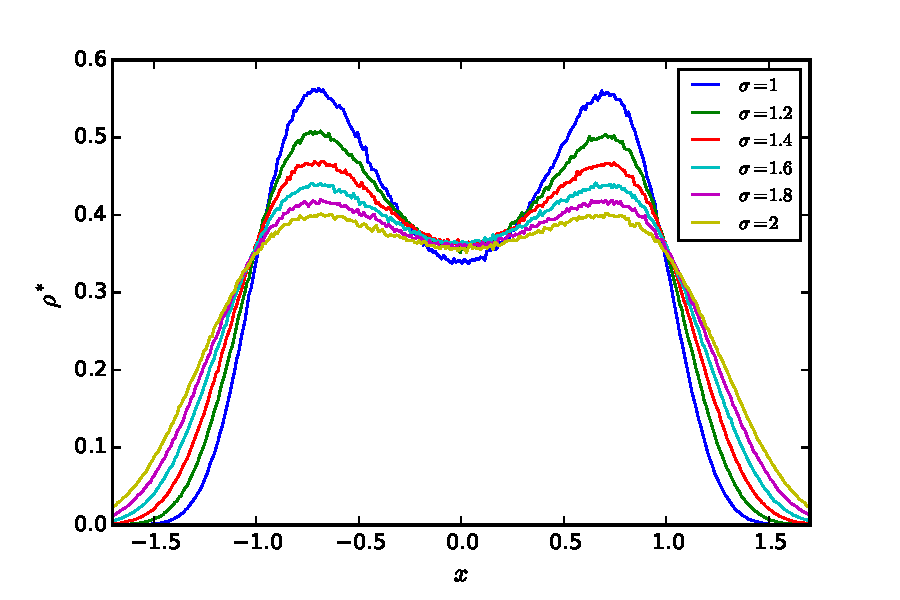
\includegraphics[width=0.49\linewidth]{../Problems/WeightedParticles/checkSystem/plots/bif/fixed_states_sde(sigma)_Ne6_mean_M10_LR}
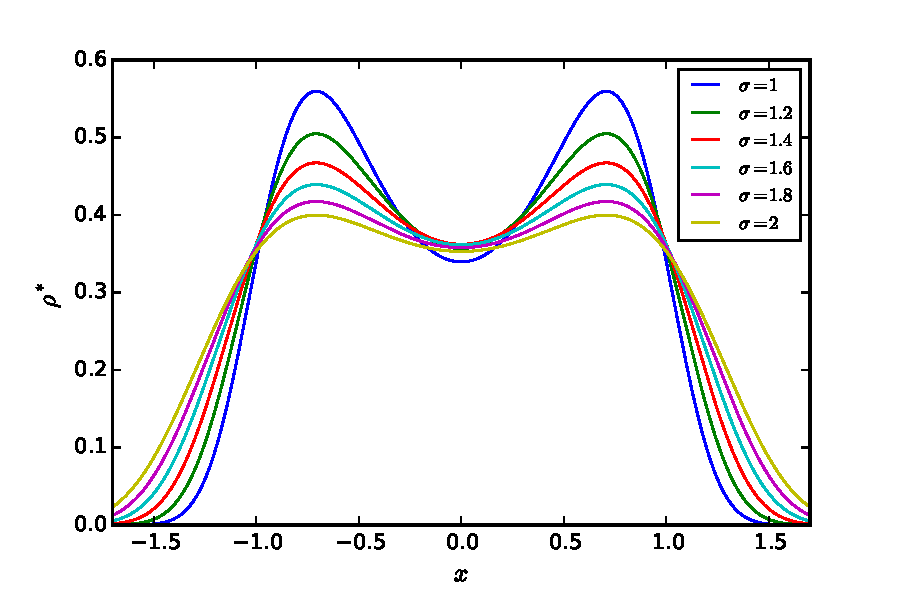
\includegraphics[width=0.49\linewidth]{../Problems/WeightedParticles/checkSystem/plots/bif/fixed_states(sigma)_analytic}
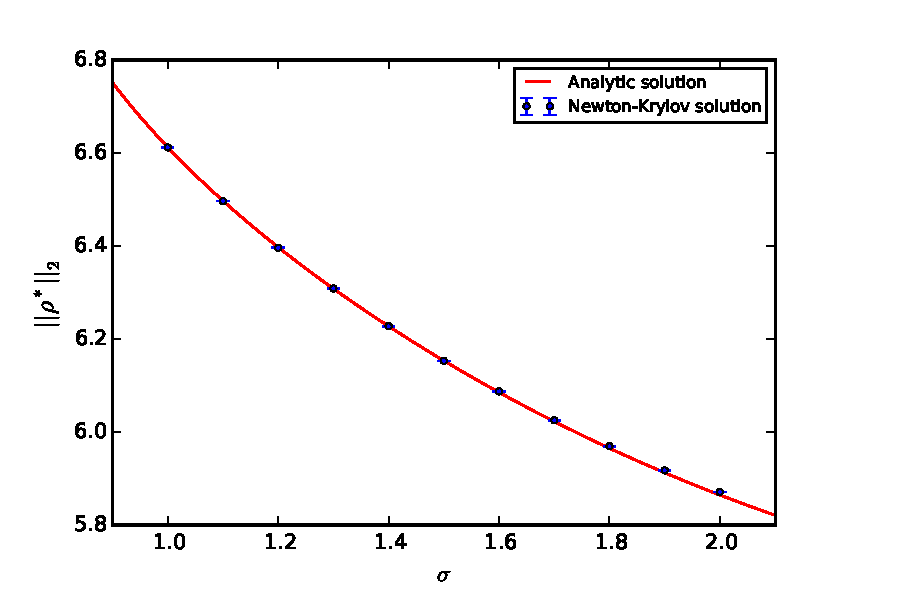
\includegraphics[width=0.9\linewidth]{../Problems/WeightedParticles/checkSystem/plots/bif/bifurcation_sde_Ne6_anal(sigma)_LR}
\caption{The steady states calculated with the Newton-Krylov-solver for the SDE  (\textit{top left}) are compared with the analytical solutions (\textit{top right}). The fixed points are visualized as the 2-norm of the density, and plotted as a function of the continuation parameter $\sigma$ (\textit{bottom}). The branch of fixed points appears to be in correspondence with the 2-norm of the analytic function $\rho^*(\sigma) =  \exp{\left[-\frac{2 V(x)}{\sigma^2}\right]} $. %{\mathcal{N}} $.
Parameter values: $\Delta \sigma =0.1$, $N=10^6$, $M=10$, $\Delta t = 10^{-3}, \Delta T = 10^{-1}, \Delta x = 10^{-2}, \epsilon_{\texttt{GMRES}}=10^{-5},  \delta_{\texttt{Newton}} = 45 \cdot 10^{-5}, \varepsilon_J=10^{-5}$}.
\label{fig:fixed_states_sde(sigma)_Ne6_mean_M10_LR}
\end{figure}


\begin{figure}
\centering
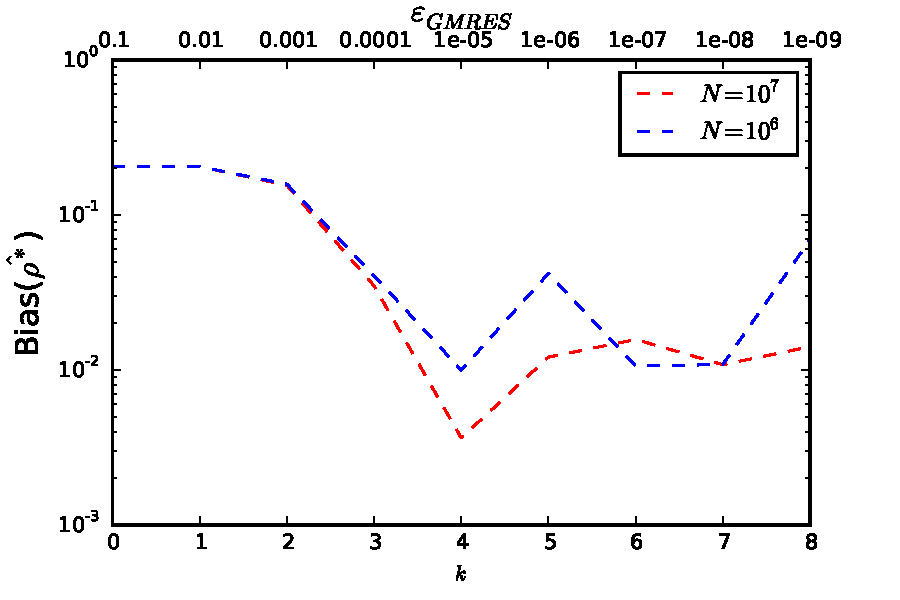
\includegraphics[width=0.7\linewidth]{../Problems/WeightedParticles/checkSystem/Newton/plots/adapt_GMREStol_every_Nstep}
\caption{}
\label{fig:adapt_GMREStol_every_Nstep}
\end{figure}



%
%\subsection{timings}
%Simulation time for solving sde, ten Newton iterations, with N=1e8, tol=1e-7: Time = 34u26m15s
%



